%%%%%%%%%%%%%%%%%%%%%%%%%%%%%%%%%%%%%%%%%%%%%%%%%%%%%%%%%%%%%%%%%%%%%%%%%%%%%%%%
%2345678901234567890123456789012345678901234567890123456789012345678901234567890
%        1         2         3         4         5         6         7         8
% THESIS CHAPTER
% \usepackage{tikz}

\chapter{Related work}
\label{chap:relatedwork}
\ifpdf
    \graphicspath{{RelatedWork/Figures/PNG/}{RelatedWork/Figures/PDF/}{RelatedTerminology/Figures/}}
\else
    \graphicspath{{RelatedWork/Figures/EPS/}{RelatedWork/Figures/}}
\fi

% short summary of the chapter
% short summary of the chapter...

% One or more chapters should be devoted to the description of the
% proposed approach...

% In particular, this chapter describes the design adopted by this research to achieve the aims and objectives stated in the Introduction.

Cover song identification has been a very active topic of research in the last
10 years. The task has spawned many solutions, so for the scope of this project
it is infeasible for each technique to be analysed in detail - from technical
implementation details to results on datasets. To fully cover the active
developments in the research area this chapter offers a summary of other related
research which is not the direct focus of the project.

The chapter is divided into two sections. The first one gives an overview of
techniques of determining identification. Second one is an analysis of the
algorithms submitted and their results for the \textit{Cover song
identification} task, part of the Music Information Retrieval Evaluation
eXchange (MIREX) conference \cite{mirex}. The format is similar to a
competition, where participating researchers submit potential solutions to a
task and each proposal is evaluated under equal conditions. The evaluation
environment is preserved throughout the MIREX editions, so results from
different years are comparable between each other.

Both studies into the field were conducted before the selection of the main
audio similarity algorithms for the project and their implementation in a
benchmark. This allowed for an informed decision on what audio features are
performing best and also ensured that algorithms not included in MIREX are
picked, to potentially present a contribution to the field.

\section{Examination of other audio similarity techniques and algorithms not analysed by the project}
\label{sec:othersimilaritytechinques}
\section{Cover song identification in MIREX 2005-2018}
\label{sec:scientificpaper}

To present and evaluate the workings on solving the cover song identification
problem in 2006 the MIREX conference created the \textit{Cover Song
Identification} task. The challenge involves an algorithm submission finding a
cover version of a query song within a dataset. The versions of the cover songs
would vary greatly in terms of genre (classical, jazz, gospel, etc.), styles and
orchestrations. The datasets used for evaluation are the MIREX 2006 US Pop Music
Cover Song dataset (1000 tracks, each track is 16-bit monophonic, 22.05 kHz
sampling rate, wav format) and, beginning 2009, the Mazurka dataset (539 tracks,
539 track queries, each track is 16bit monophonic, 22.05 kHz sampling rate, wav
format). The former dataset has 30 cover songs each represented by 11 different
versions for a total of 330 files. Each of the files are then individually run
as queries for the algorithms. Each algorithm then attempts to return the other
10 versions of the same song.  The latter dataset consists of mazurka dance
music. Because of that 11 versions from 49 mazurkas are randomly picked (and
thus 539 tracks are taken from the full set). Afterwards a 539x539 distance
matrix is created which gives the ranks of each of the associated cover
versions. The only output the submitted algorithms should return is a
\textit{number of queries} $\times$ \textit{number of candidates} distance
matrix. The task specification is taken from MIREX 2018 \cite{mirex:2018}.
Information about winning participants and their ranking could be found under
\ref{subsec:resultseval}.

\subsection{Examined work}
\label{subsec:examinedwork}
Out of the 40 submissions related to the cover song task in the MIREX conference
25 were considered. There are 15 papers missing from the MIREX website and are
therefore excluded from this report. The missing submissions also unfortunately
include winners of the challenge in 5 different years. The cover song algorithms
were analysed to outline the most used techniques for capturing audio features
suitable for determining similarity. The similarity metrics themselves were also
examined.

From the work examined 5 of the papers present improvements to previous submitted algorithms. That makes the overall number of unique algorithms inspected to 20.
\subsection{Results evaluation}
\label{subsec:resultseval}

In order to determine which algorithms perform best we need to look at the
results achieved each year. From them we would then be able to determine what
audio similarity techniques have worked best so far and examine them further in
depth. 

The results outlined here are based on the statistics provided by MIREX each
year for the results of the cover song identification task. Each year MIREX
publishes the total number of covers identified (TNCI), the mean number of
covers identified (MNCI), the mean of average precisions (MAP) and the mean rank
for first correctly identified cover (MRFCIC) for each algorithm. The results
include the algorithms for which the corresponding paper is missing. 

Let us look at the best THCI results plotted over the years for the MIREX cover
song identification task:

\begin{figure}[H]
    \centering
    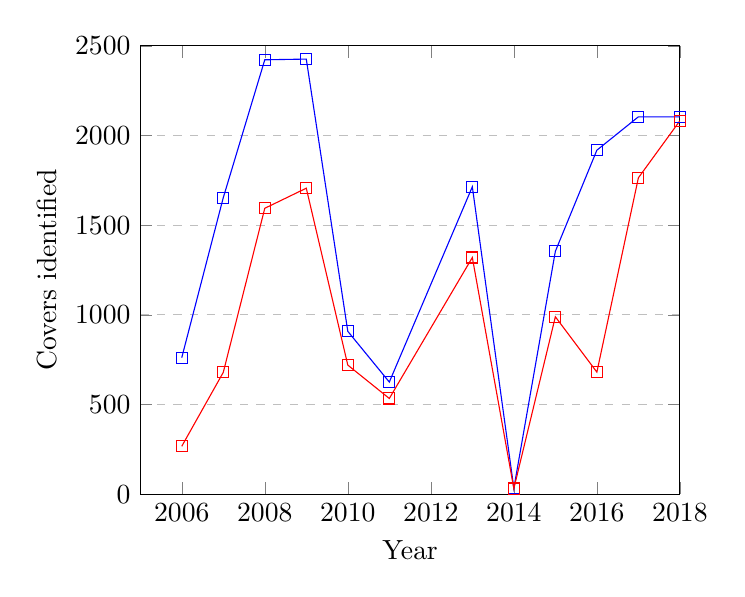
\begin{tikzpicture}
        \begin{axis}[
            /pgf/number format/.cd,
            1000 sep={},
            title={},
            xlabel={Year},
            ylabel={Covers identified},
            xmin=2005, xmax=2018,
            ymin=0, ymax=2500,
            % xtick={2006, 2008, 2010, 2012, 2014, 2016, 2018},
            xtick={},
            ytick={},
            legend pos=north west,
            ymajorgrids=true,
            grid style=dashed,
        ]
         
        \addplot[
            color=blue,
            mark=square,
            ]
            coordinates {
            (2006,761)(2007,1653)(2008,2422)(2009,2426)(2010,908)(2011,625)(2013,1714)(2014,33)(2015,1354)(2016,1918)(2017,2104)(2018,2104)
            };
            % \addlegendentry{Max THCI}
        \addplot[
            color=red,
            mark=square,
            ]
            coordinates {
            (2006,266.875)(2007,678.875)(2008,1593.875)(2009,1706)(2010,719.666666666667)(2011,533.5)(2013,1319.5)(2014,31)(2015,989)(2016,680.2)(2017,1763.75)(2018,2082)
            };
            % \addlegendentry{Average THCI}
            \end{axis}
        \end{tikzpicture}
    \caption[THCI of winning submissions in MIREX 2005-2018]{Results of the winning submissions in the period 2005-2018. The blue line represents the max THCI achieved for each year (i.e. the challenge winners). The red line outlines the average THCI for each year the task has taken place. The challenge did not run in 2005 and 2012.}
    \label{fig:mirex_results}
\end{figure}

We could see that the best performing submissions are the ones published in
2008, 2009 and 2018. It also seems that between 2009 and 2017 no significant
improvement has been achieved. Based on that we could establish two imaginary
'periods' in the challenge. If we set a threshold of 1500 average covers
achieved we could see that this boundary outlines two groups of submissions. One
of them includes the years 2008-2009 and 2017-2018 - the 'strong' period, where
on average the algorithms perform better than the rest of the results. The
'weak' period is between 2010-2016, where we can even observe the biggest dip in
the results - in 2014 the max THCI was 33 covers identified, out of 2
submissions. We use the strong period to give us a notion about techniques that
perform well in the cover song identification task. 

To determine if there is a tendency into what type of audio feature is used, a
table comprising of all audio features used is compiled from the available
submissions:
\begin{figure}[H]
    \centering
    \scalebox{0.90}{
    \begin{tabular}{c|c|c}
        \textbf{Audio feature} & \textbf{Times used} & \textbf{Winner} \\
        \hline
        Chroma features & 12 & 2006, 2018 \\
        % HPCPs & 5 & 2007, 2008, 2009, 2016 \\
        % MFCCs & 2 & \\
        Harmonic Pitch Class Profiles (HPCPs) & 5 & 2007, 2008, 2009, 2016 \\
        Mel-frequency cepstral coefficients (MFCCs) & 2 & \\
        HPCP, MFCC and MFCC SSM combined & 1 & \\
        Basic Pitch Class Profiles (PCP) & 1 & \\
        Custom technique & 1 & 2014 \\
        Relationship (distance) to other songs in set & 1 & \\
        Statistical Spectrum Descriptors & 1 & \\
        Pitch line estimation & 1 & \\
    \end{tabular}
    }
    \captionof{figure}[Audio feature frequency usage in MIREX 2005-2018]{Number of times a type of audio feature is used in MIREX 2005-2018. The \textit{Winner} column indicates whether the best algorithm for the year utilises the feature.}
\end{figure}

Unfortunately only 7 out of the 13 winning papers were available online, so it
is unclear whether they are also using any of the features for information
extraction. It is worth noting that the winning submissions from 2007, 2008 and
2009 are evolutions of the same algorithm \cite{serra2007cover}
\cite{serra2008improving} \cite{serra2009cover}. The \textit{custom technique}
mentioned in the table refers to an algorithm implementing a non-conventional
audio feature which achieves the worst winning result in the MIREX competition
so far  -  only  33  covers  identified  (out  of  3300 possible).

Some of the main audio similarity algorithms explored in the project use chroma
features and MFCCs as audio features. Therefore in this section we only explore
the structure of HPCPs.

\subsection{Harmonic Pitch Class Profiles}
\label{subsec:hpcp}

For each pitch representing a semitone part of an equal temperament scale a
\textit{pitch class} is the set of all pitches which are all separated by an
octave from each other. Knowing that we can create a \textit{pitch class profile
(PCP)} - a vector which represents the intensities of all twelve pitch classes
\cite{fujishima1999real}. PCPs become \textit{harmonic} when they represent the
relative intensities of the pitch classes within an analysis frame in a signal
\cite{wiki:hpcp}. Straying from the general definition of a PCP they could also
be extracted over a 24 or 36-bin pitch spectrum, representing the relative
intensity of every 1/2 or 1/3 semitones respectively.

HPCPs are generally extracted using a Fourier transform to determine the
constituting frequencies in the audio stream. The resulting spectrogram is then
filtered to include only an audible spectrum of frequencies, which are then
mapped to their pitch classes. Each time frame is then normalised to obtain the
HPCP audio feature representation of a song.